\chapter{Prehľad algoritmov}
Na hľadanie najkratších ciest v grafe poznáme mnoho algoritmov, ktoré vieme rozdeliť do troch skupín.


\begin{itemize}
\item Point To Point Shortest Path(P2PSP) - hľadajú najkratšiu cestu medzi dvoma zadanými bodmi
\item Single Source Shortest Path(SSSP) - pre daný vrchol {\sl v} hľadajú najkratšiu cestu do všetkých vrcholov grafu.
\item All Pairs Shortest Path (APSP)- skúmajú najkratšiu cestu medzi všetkými dvojicami vrcholov.
\end{itemize}

Tieto problémy sú na obecných grafoch NP-ťažké.
Napriek tomu na mriežkových grafoch (kde sú vzdialenosti medzi vrcholmi vždy kladné) existujú algoritmy v polynomiálnom čase.

V práci budeme ďalej zaoberať riešením prvého problému (Point to Point Shortest Path). 

V tejto kapitole popíšeme algoritmy, ktoré sú použiteľné na grafoch s nezápornými dĺžkami hrán. TODO?? prerob

TODO?? POTIAL VSETKO PREPISANE a myslim, ze clekom prijemne citatelne.

\section{Dijkstrov algoritmus}
Medzi základné algoritmy typu SSSP patrí Dijkstrov algoritmus \cite{dijkstra59} popísaný už v roku 1959. 
Miernu modifikáciu pôvodného algoritmu môžeme vidieť na (Algoritmus \ref{alg:dijkstra}).  ASK?? spravil som citacie spravne?
Patrí medzi relaxačné algoritmy a zbehne korektne na grafoch
s nezápornými hranami.

Pri hľadaní cesty z vrcholu $s$ do vrcholu $t$ prechádzame postupne vrcholy s neklesajúcou vzdialenosťou od $s$, až dokým sa nedostaneme k cieľovému vrcholu $t$.



Vizuálne si beh algoritmu môžme predstaviť ako kruh so stredom v bode $s$ so zväčšujúcim sa polomerom.

?? rozlisujeme tri stavy vrcholov, co je halda blablabla

\begin{algorithm}
\caption{Dijkstra: nájdi najkratšiu cestu medzi dvoma bodmi $s$ a $t$}
\label{alg:dijkstra}
\begin{algorithmic}[1] % number one = line numbering is on
\REQUIRE graf $G$
\ENSURE hodnotiaca funkcia $h$ obsahujúca najkratšie cesty  z vrcholu $s$ do vrcholov grafu


\STATE $ h(*) \leftarrow \infty $
\STATE $ stav(*) \leftarrow$ NENAVŠTÍVENÝ

\COMMENT {pridám počiatok}
\STATE $h(s) \leftarrow 0$
\STATE $stav(s) \leftarrow $ OTVORENÝ
\STATE Heap $H$
\STATE $Insert(H, s)$

\WHILE {$H$  not empty}
	
	\STATE // vyberiem v -- najbližší otvorený vrchol
	\STATE $v \leftarrow ExtractMin(H)$
	
	\WHILE {$stav(v) \neq $ OTVORENÝ}
		\STATE $v \leftarrow ExtractMin(H)$
	\ENDWHILE
	
	\STATE // zrelaxujeme vrchol $v$
	\FORALL {$e$, $e = (v, u)$}
		\IF {$h(u) \textgreater h(v) + l(v, u)$}
			\STATE $Insert(H, v)$
			\STATE $stav(u) \leftarrow$ OTVORENÝ
			\STATE $h(u) \leftarrow h(v) + l(v, u)$
			
		\ENDIF
	\ENDFOR
\ENDWHILE

\end{algorithmic}
\end{algorithm}

\begin{theorem}
V dijkstrovom algoritme uzatvárame každý dosiahnuteľný vrchol práve raz.
\end{theorem}
ASK?? citovat dijkstru a maresa ako dokaz? 

\subsection{Zložitosť}
Na každý vrchol zavoláme operáciu $Insert$ maximálne $deg(v)$-krát a teda počet všetkých zavolaní tejto operácie bude rádovo $\BigO{\sum_{v}{deg(v)}} = \BigO{m}$.
Zo štruktúry môžme vybrať maximálne toľko prvkov, koľko sme tam vložili a teda aj volania $ExtractMin$ trvajú $\BigO{m}$.

Algoritmus teda zbehne v čase $\BigO{m T_i + m T_e}$, kde $T_i$ odpovedá času na vloženie prvku a $T_d$ odpovedá času na vybranie najmenšieho prvku.

To znamená, že zložitosť algoritmu závisí od zložitosti operácií $Insert$ a $ExtractMin$. Na riedke grafy je obecne v praxi najvýhodnejšie použiť 
binárnu haldu, ktorej obe operácie trvajú $\BigO{\log{n} } $ a celkový čas je teda $\BigO{m\log{n}}$
Prehľad štruktúr aj so zložitosťami operácií $Insert$ a $ExtractMin$ sa nachádza napr. na \cite{mares07}.

\subsection{Halda na mriežkovom grafe}
Nakoľko mriežkový graf je veľmi špeciálny typ grafu,
vieme niektoré jeho vlastnosti využiť na to, aby sme vytvorili štruktúru, ktorá zvládne obe operácie v konštantnom čase. 


Na konštrukciu tejto štruktúry (viď \cite{gs97}) budeme potrebovať nasledujúcu vetu.

\begin{theorem}
Pokiaľ sme v Dijkstrovom algoritme uzavreli vrchol $u$ so vzdialenosťou $d_u$ a najkratšia hrana v grafe má dĺžku $\epsilon$, tak môžme taktiež 
uzavrieť všetky vrcholy $v$ so vzdialenosťami $d_v \in (d, d + \epsilon)$.
\end{theorem}
\begin{proof}
Do haldy vieme pridávať len vrcholy so vzdialenosťami aspoň $d + \epsilon$ (kratšia hrana tam už nie je), 
ale~tie už cestu k~vrcholom so~vzdialenosťami
$d_v \in (d, d + \epsilon)$ skrátiť nemôžu.
\end{proof}


Keďže dĺžka najkratšej hrany $\epsilon = 1$, tak v štruktúre budeme mať priehradky, ktorých rozsah je ostro menší ako $\epsilon$. 



Na konštrukciu lineárneho Dijkstrovho algoritmu potrebujeme priehradkovú haldu. Tá vie vybrať  \uv{jeden z najmenších} prvkov.
v konštantnom čase a rovnako ako aj vložiť prvok.

\begin{figure}[h]
\centering
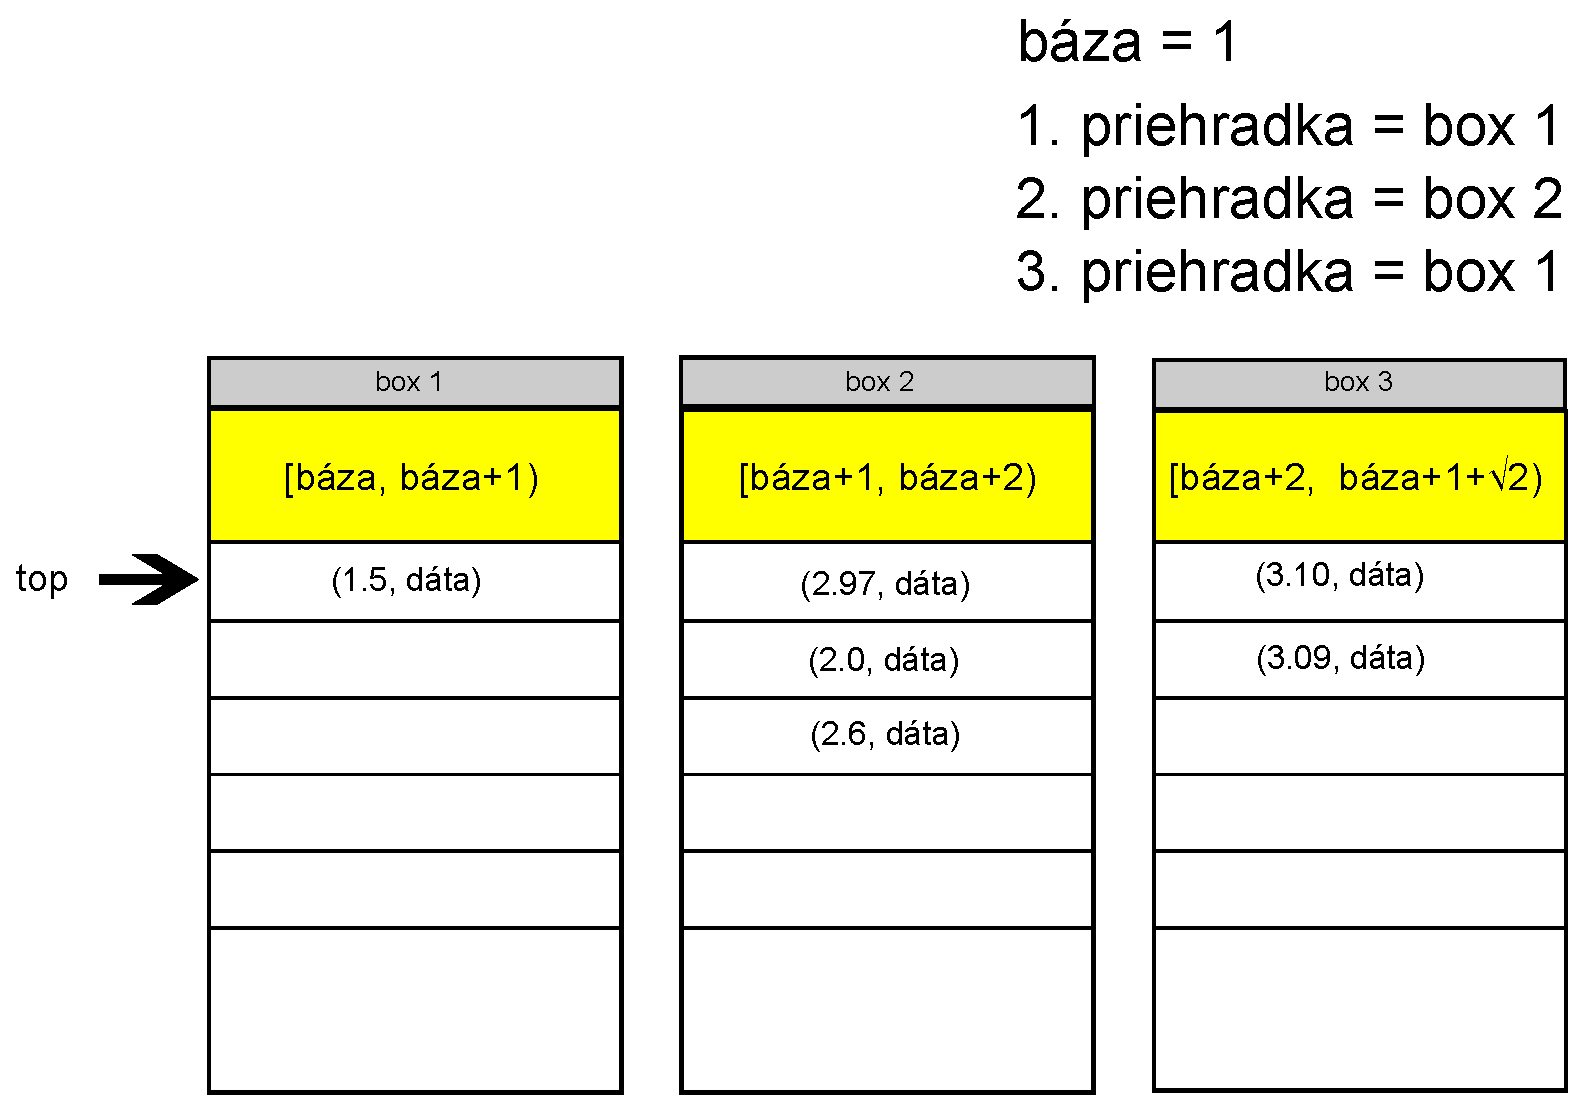
\includegraphics[width=\textwidth]{./img/priehradky_naplnene_default.eps}
\caption{Priehradky}
\label{fig:priehradky}
\end{figure}


\begin{figure}[h]
\centering
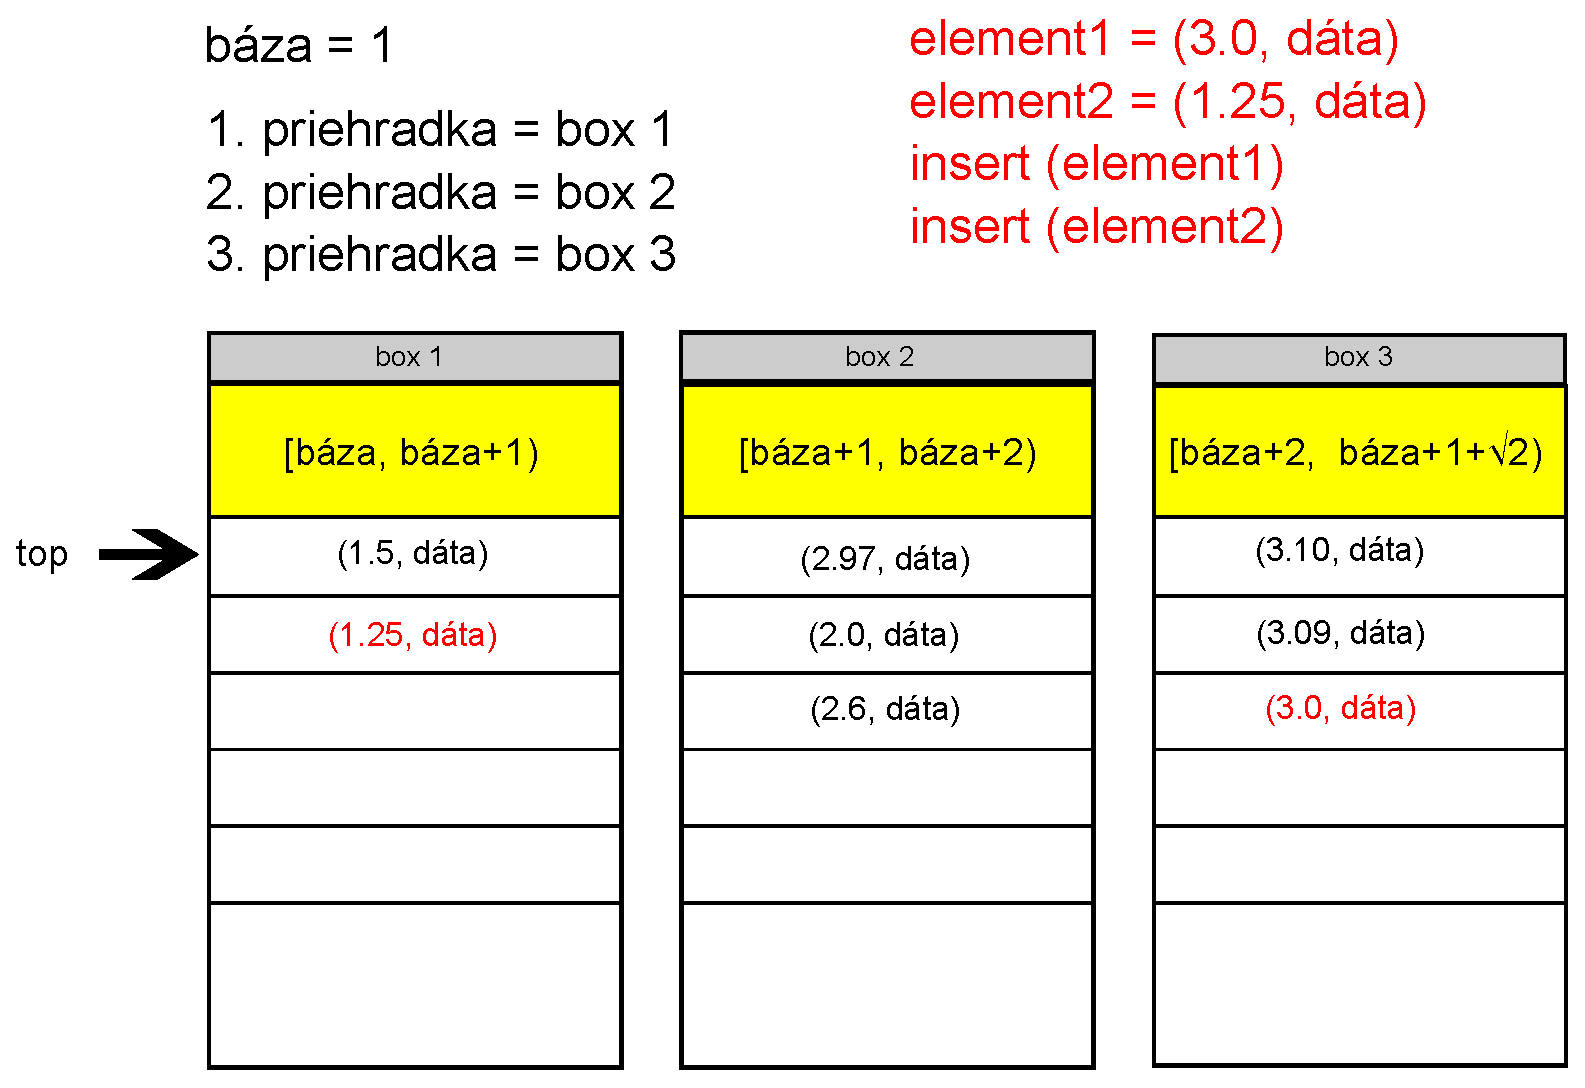
\includegraphics[width=\textwidth]{./img/priehradky_naplnene_default_i.eps}
\caption{Insert}
\label{fig:priehradky_i}
\end{figure}

\begin{figure}[h]
\centering
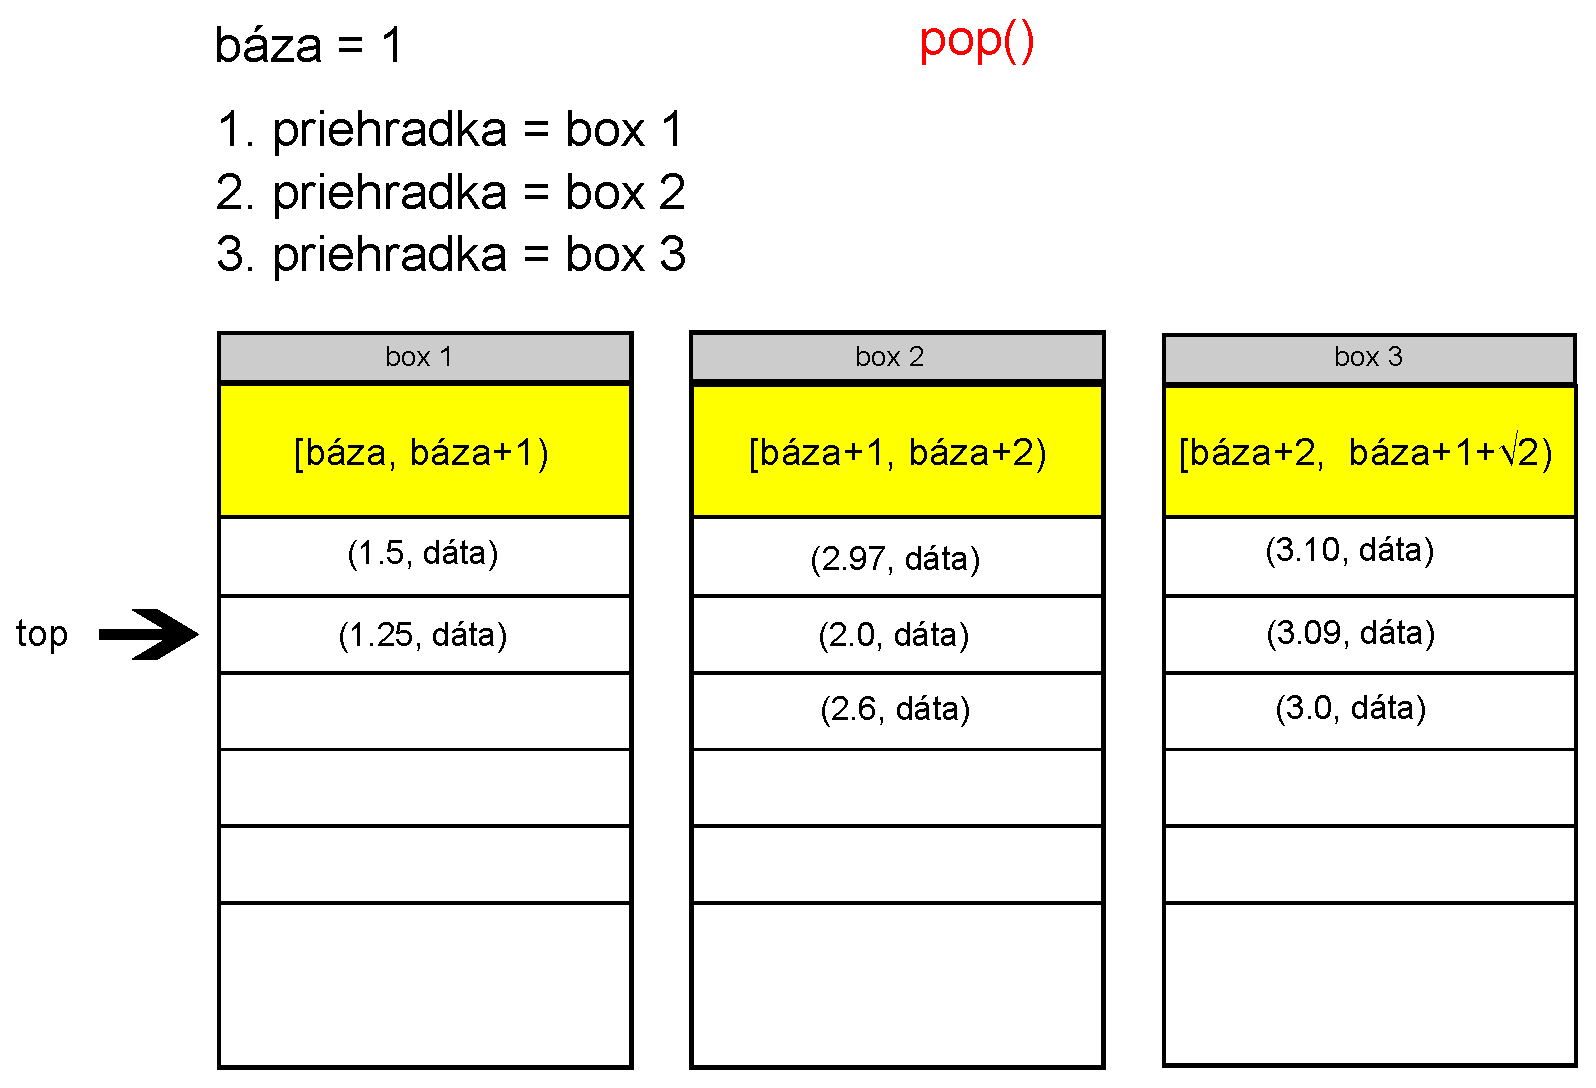
\includegraphics[width=\textwidth]{./img/priehradky_naplnene_default_i_d1.eps}
\caption{Insert}
\label{fig:priehradky_i_d1}
\end{figure}

\begin{figure}[h]
\centering
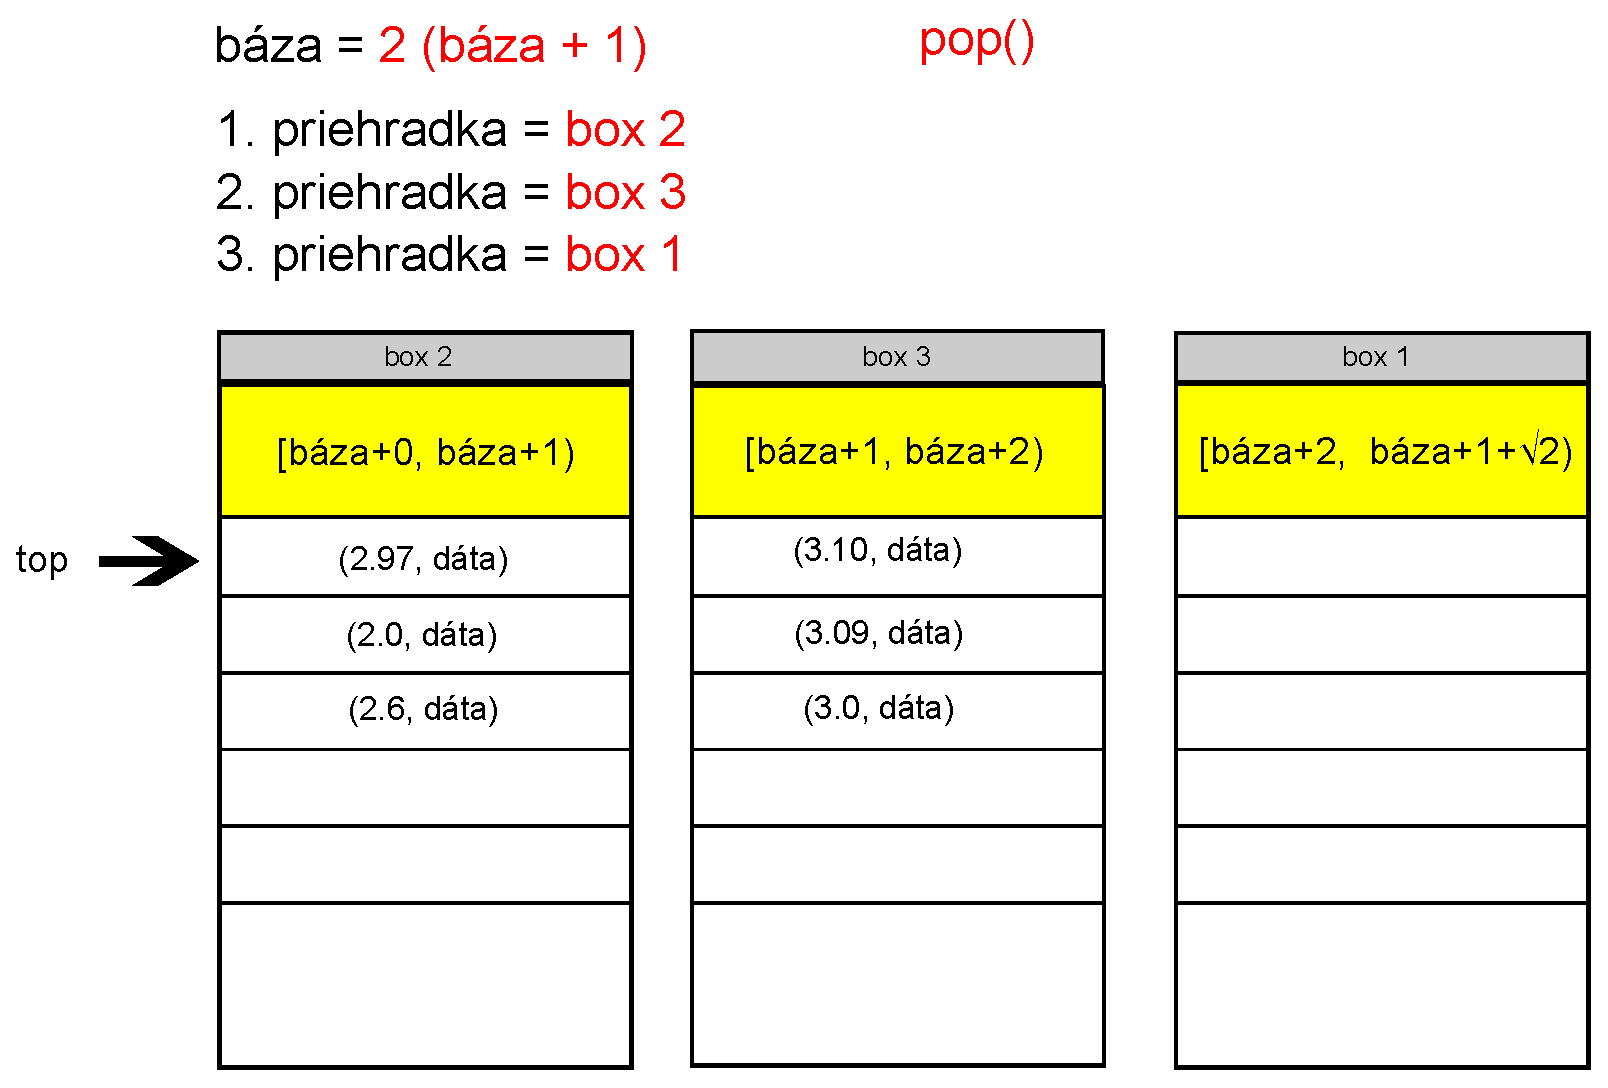
\includegraphics[width=\textwidth]{./img/priehradky_naplnene_default_i_d2.eps}
\caption{Insert}
\label{fig:priehradky_i_d2}
\end{figure}

blablabla


\section{A*}
dalsi algoritmus do zbierky je a* \cite{astar72}.
